%!TEX root = ../../lod-group1.tex
\subsection{System Architecture}
\label{subsec_method_architecture}

The architecture of \emph{Match Forrest, Match!} is shown in Figure \ref{fig_architecture}.

The central component of the system is the \textit{Task Distributor}.
This component is responsible for managing the other components, \textit{Crawler}, \textit{Triplifier}, \textit{Updater} and \textit{Matcher and Merger}.
Therefore, it uses a messaging system, explained in Section \ref{subsubsec_messaging_infrastructure}.

In general, the first step to get a movie into the system is to get the actual movie resource.
This step is executed by the \textit{Crawler.}
This component is responsible for downloading websites and for sending requests to the provided API from a data source.

Once the page is downloaded, the \textit{Triplifier} can triplify the resource.
This means, it extracts the information from the resource and creates triples out of it.
Therefore, the ontology, defined in Section \ref{subsec_method_ontology}, is used.

The component \textit{Matcher and Merger} is in charge of matching two movies from different data sources, so they only can be found once in the resulting dataset.
This component is explained in detail in Section \ref{subsec_method_matching}.

The updater, described in Section \ref{subsec_method_updating}, ensures that the existing movies are always up to date and that new movies are in the system.

The triple store \textit{Virtuoso} is used to store the resulting triples.
To distinguish between the sources of the different triples, triples from a data source are stored in a graph named after the source.
Thus, there are four graphs in the triplestore, IMDb, Freebase, TMDb and OFDb.

\begin{figure}[ht]
  \begin{center}
  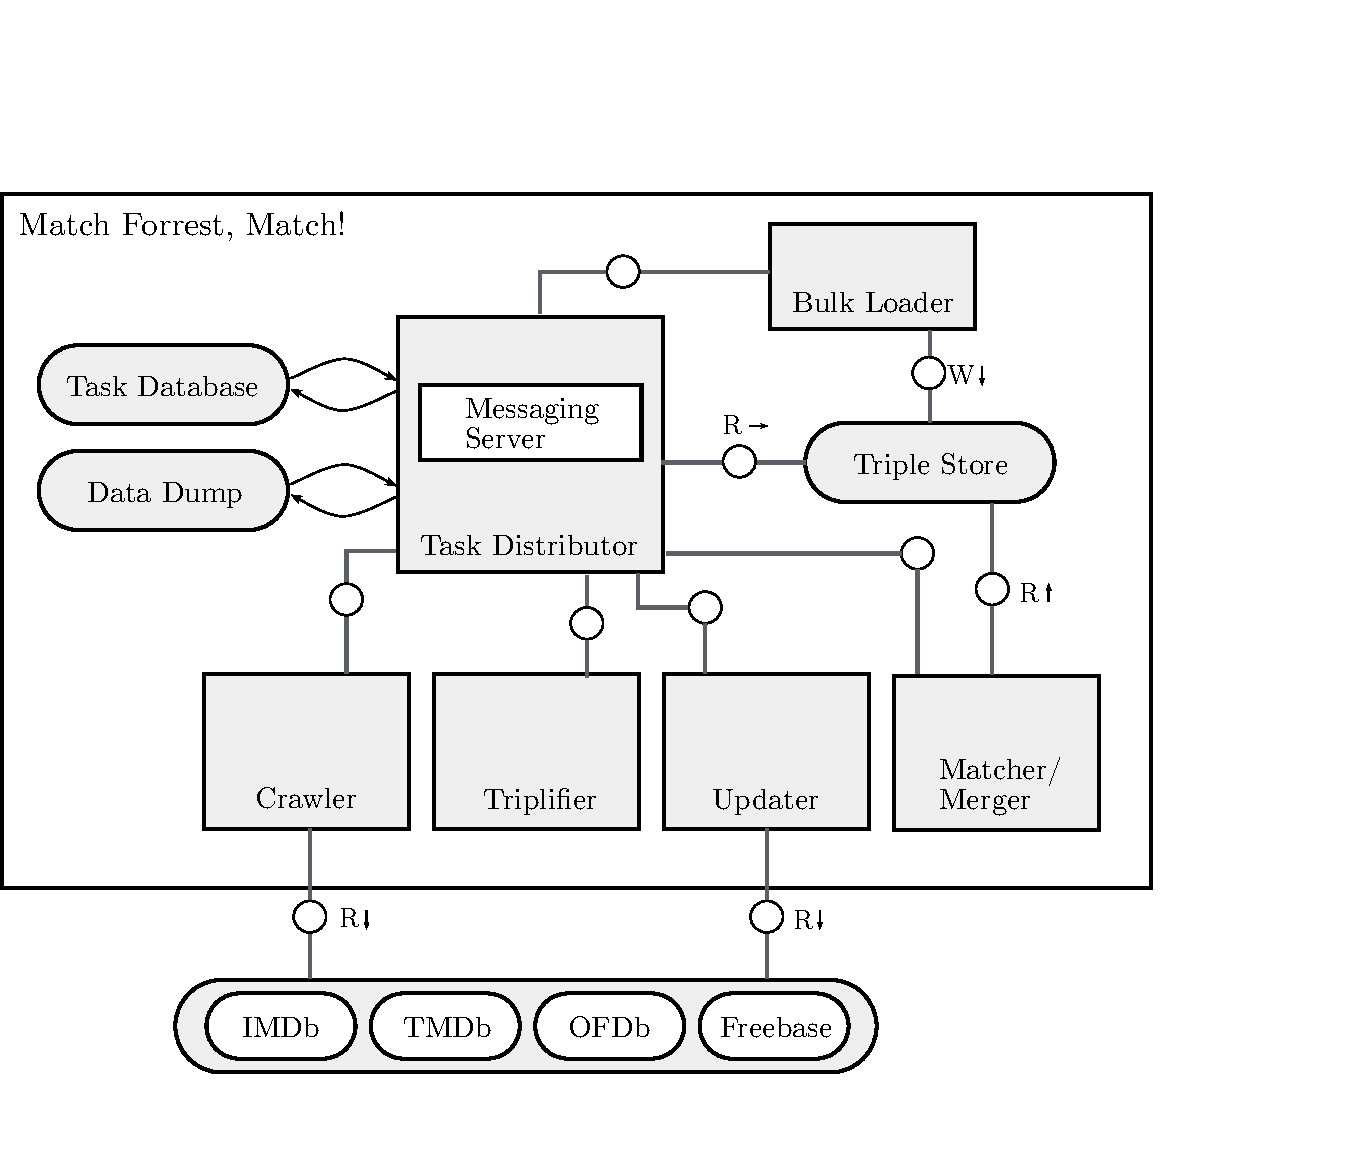
\includegraphics[width=0.85\textwidth]{images/architecture.pdf}
  \end{center}
  \caption{Architecture}
  \label{fig_architecture}
\end{figure}

\subsubsection{Messaging Infrastructure}
\label{subsubsec_messaging_infrastructure}

%TODO Stefan, Dominik verifizieren

The process of crawling, triplifying and matching a movie resource takes a lot of time.
Especially there are limits to crawl some web pages, which means that waiting times can occur. Triplifying and matching needs computational resources.
Because the steps can be done in parallel, a messaging infrastructure was implemented to speed up the process and to avoid crawl limits.

%The messaging infrastructure is based on \emph{RabbitMQ}\footnote{\url{http://www.rabbitmq.com/}}.
Therefore the \textit{Task Distributor}, including the messaging server, uses \emph{RabbitMQ}\footnote{\url{http://www.rabbitmq.com/}} to coordinate and send created task to multiple workers.

A task consists of the following fields
\begin{itemize}
  \item \textbf{Id}:
  The unique id of the task.
  \item \textbf{Task type}:
   The type of the task.
  Basically it exists a type for each of the compontent, controlled by the \textit{Task Distibutor}, for example ``Triplify'' or ``MatchAndMerge''.
  ``Triplify'' is a task execute by the \textit{Triplifier} component.
  The \textit{Matcher and Merger} component works on ``MatchAndMerge'' tasks.
  There are also tasks, which combine some steps, such as the ``CrawlifyMatch'' task, which crawls, triplifies and matches a movie.
  \item \textbf{Due date}:
  The date until when the task should be finished.
  \item \textbf{file or url}:
  The file or url which is needed to execute the task.
  \item \textbf{Finished:}
  Defines, if the task is already done.
  \item \textbf{Graph}:
  The graph in which the resulting triples should be stored.
  \item \textbf{Remarks}:
  Additional information needed when executing a task.
  For example, it could tell weather a certain entity should be delete from the triple store before storing new triples.
\end{itemize}
Not all fields have to be set, it depends on the task type, which fields are needed.
For example the ``Triplify'' task needs a file, but the ``MatchAndMerge'' task does not.

All tasks are stored in a SQL database and new ones are created by the \textit{Updater}.
To get an initial data set tasks have to be created manually.

The messaging server takes a task out of the SQL database and puts it into the messaging queue.
The functionality of the messaging system, is shown in Figure \ref{fig_messaging_infrastructure}.
A worker, which is registered on the task queue, gets the new task pushed.
If multiple workers are registered, a free worker is selected by using the round robin principle to perform the next task.
When the worker has finished the task, it sends his answer to the answer queue and waits for the server to acknowledge his work.
The server gets the answer of the worker from the answer queue and stores given triples into the triple store and files to the file system.
When the answer was successfully stored, the server sends his acknowledgement to the worker, who forwards the acknowledgement to the task queue.
The task is now successfully executed and the worker can work on the next task in the task queue.
If an acknowledgement takes longer than a given time, the task would be given to another worker again.
This assures that no task get lost.

\begin{figure}[ht]
  \begin{center}
  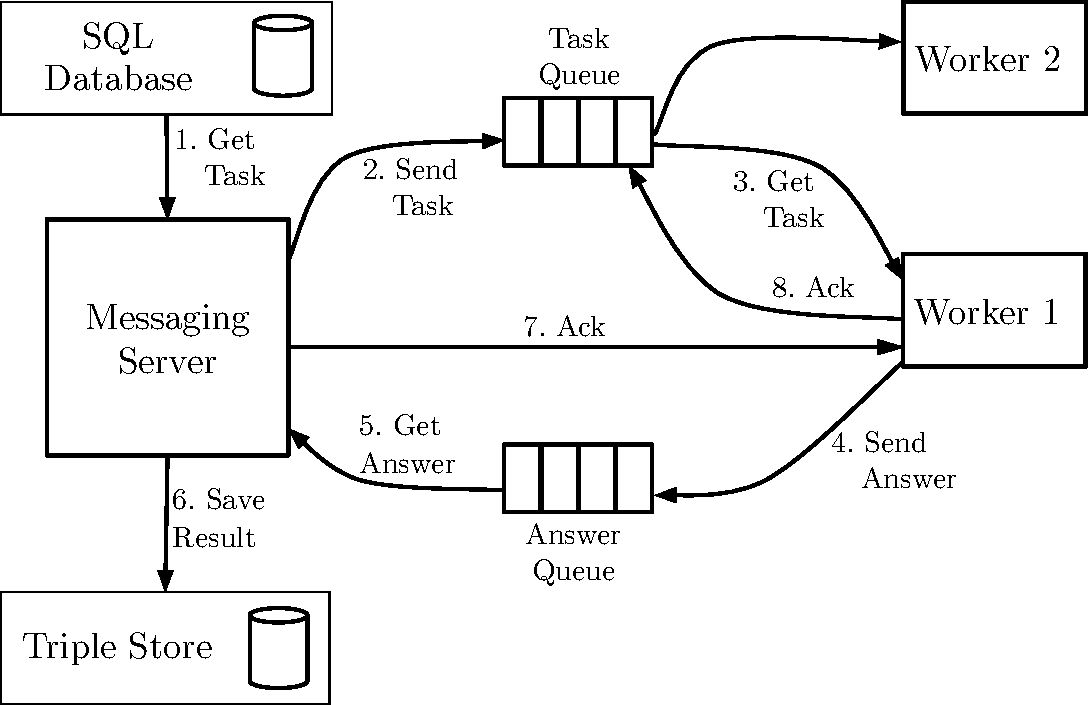
\includegraphics[width=0.8\textwidth]{images/rabbit_mq.pdf}
  \end{center}
  \caption{Messaging Infrastructure using RabbitMQ}
  \label{fig_messaging_infrastructure}
\end{figure}